% filename: HEP_GL_OperationSafetyConcept

\documentclass{article}

\usepackage[utf8]{inputenc}
\usepackage[top=3cm, headheight=2.2cm, headsep=10pt]{geometry}
\usepackage{graphicx}

% To reference the last page
\usepackage{lastpage}

% Like `tabularx` but supports pagebreaks
\usepackage{ltablex}
% Adjust row vertical spacing
\renewcommand{\arraystretch}{1.2}

% Multiline cells
\usepackage{makecell}

% Set date format to ISO 8601
\usepackage{datetime}
\newdateformat{isodate}{\THEYEAR-\twodigit{\THEMONTH}-\twodigit{\THEDAY}}

% Table colouring
\usepackage[table,dvipsnames]{xcolor}
\definecolor{tableHeaderColor}
{rgb}{0.75,0.75,0.75}
\definecolor{tableColumnColor}
{rgb}{0.95, 0.95, 0.95}
\definecolor{notesColor}
{rgb}{0.95, 0.95, 0.95}
\definecolor{highlightColor}
{rgb}{1.00, 0.95, 0.80}

% Icons for checkbox
\usepackage{pifont}

% Command to create a checkbox
\newcommand{\checkbox}{\ding{113}}

% For automatic counters
\usepackage{array}

% Header and footer
\usepackage{fancyhdr}
\pagestyle{fancy}
\fancyhf{} % Clear header and footer
\renewcommand{\headrulewidth}{0pt}
\lhead{\includegraphics[width=2cm]{../../common/assets/HELIOS_LOGO.png}}
\rhead{\includegraphics[width=2cm]{../../common/assets/ARIS_space_to_grow_LOGO-black.pdf}}
\cfoot{\thepage}
\fancyfoot[L]{Project HEPHAESTUS}
\fancyfoot[C]{Page \thepage\ out of \pageref{LastPage}}

% Draft watermark
\newboolean{isDraft}
\setboolean{isDraft}{true} % Set to false to remove the watermark
\ifthenelse{\boolean{isDraft}}{
  \usepackage{background}
  \backgroundsetup{
    scale=25,
    color=gray,
    opacity=0.4,
    angle=45,
    position=current page.center,
    contents={Draft}
  }
}{}

% Highlight colour
\usepackage{soul}
\sethlcolor{magenta}

% Strikethrough
\usepackage[normalem]{ulem}

% Clickable Hyperlinks
\usepackage[colorlinks=true, linkcolor=blue, urlcolor=blue]{hyperref}

% Toggleable procedure items
\usepackage{etoolbox}



\title{Operation Safety Concept}
\author{Guideline}
\date{Version: \isodate\today}

\begin{document}

\maketitle

% Set the page style for the title page
\thispagestyle{fancy}

\section{Scope}

Within the framework of ETH Focus Project HEPHAESTUS, a Liquid Rocket Engine firing campaign is performed on the Dübendorf Airfield. The team members of project HEPHAESTUS received the permission from the Airfield to perform their tests. To ensure efficient and safe tests, this operational safety concept shall describe the test area and its available safety equipment and should give advice on how to behave during procedures and in emergencies.  
\\ \noindent
This document shall be read before each testing day by every visitor. 
With their signatures on the document HEP\_GL\_SafetySignature, all attendees confirm their knowledge of the general safety precautions and rules of behaviour according to this document. 

\section{Location of safety-relevant Institutions}
The contact information of the relevant safety institutions is listed in \ref{tab:safety-relevant-institutions}.
\begin{table}[h]
    \caption{Information of safety-relevant institutions}
    \label{tab:safety-relevant-institutions}
    \begin{tabularx}{0.9\textwidth}{|X|X|X|}
        \hline
        \rowcolor{tableHeaderColor} \textbf{Description} & \textbf{Address} & \textbf{Phone Number} \\ \hline
        Test Location & \begin{minipage}[t]{\linewidth}
            Flughafen Dübendorf – Hunter Stübli \\
            Rechweg \\
            8600 Dübendorf
            \vspace{1mm}
        \end{minipage} & - \\ \hline
        Spital Uster & \begin{minipage}[t]{\linewidth}
            Brunnenstrasse 42 \\
            8610 Uster
            \vspace{1mm}
        \end{minipage} & +41 44 911 11 11 \\ \hline
        Airfield Responsible & Roger Gisler & \begin{minipage}[t]{\linewidth}
            +41 58 481 79 18 \\
            If not reachable try: \\
            +41 79 944 42 52
            \vspace{1mm}
        \end{minipage} \\ \hline
        President ARIS & Chloé Pilloud & +41 79 226 39 42 \\ \hline
        Technical Advisor & Bruno Berger & +41 79 209 39 27 \\ \hline
    \end{tabularx}
\end{table}

In table \ref{tab:emergency-numbers} the emergency numbers are listed. Call them first before calling other relevant security institutions. In the case of an emergency, follow the contingency procedures as described in Section \ref{emergency-behaviour}.
\begin{table}[h]
    \caption{Emergency Numbers}
    \label{tab:emergency-numbers}
    \begin{tabularx}{0.9\textwidth}{|X|X|}
        \hline
        \rowcolor{tableHeaderColor} \textbf{Description} & \textbf{Phone Number} \\ \hline
        Ambulance & 144 \\ \hline
        Rega & 1414 \\ \hline
        Fire service & 118 \\ \hline
        Police & 117 \\ \hline
        Toxics & 145 \\ \hline
    \end{tabularx}
\end{table}
\section{Phases}
As scheduled in the Firing Conduction, every test is divided into the following phases:
\begin{enumerate}
    \item Pre-Preparation
    \item Preparation and Assembly
    \item Briefing
    \item Transfer to Airfield
    \textcolor{red}{
    \item Installation and Pre-Firing Checks
    \item Filling and Ignition Test
    \item Safe State Establishment}
    \item Post Firing Checks and Deinstallation
    \item Transfer to IPZ
    \item Disassembly and Inspection
    \item Debriefing
\end{enumerate}
The beginning of every phase needs to be clearly communicated to all attendees by the test conductor. Visitors shall keep a safe distance from the trailer during all phases. \\
\noindent
During phases 5 to 7, the system is in a dangerous state. Therefore, no one is allowed to leave the Hunter Stübli or designated area unless instructed to do so by the test conductor in order to execute a specific task.

\newpage

\section{Risk Assessment}
Firing tests involve pressurized systems, cryogenic and flammable fluids, as well as high temperatures and therefore have inherent risks associated with them. The risks are assessed and mitigated as described below:
\subsection{Overpressure}
An overpressure of the system can lead to rupture of components and therefore to an explosion. Overpressure can cause injury to personnel, namely hearing damage, lung damage and even death, and damage to surrounding facilities. However, during all operations with the trailer, the pressure is limited to 60 bar and all components of the system have previously been tested to 60 bar. Additional preventive measures are taken to minimise the chance of occurance and damage caused by a possible overpressure event:
\begin{itemize}
    \item Every potentially closed section of the system is equipped with a pressure relief valve, which are set to open at 80 bar. This ensures that the pressure in the system is limited to 80 bar, even in the case a pressure reducer were to fail or trapped LOX were to start evaporating. While this is higher than what the components have been tested to on the OSS side, all components are rated for at least 180 bar, which leaves a safety margin against plastic deformation of 2.25.
    \item The TNT equivalent of the potential energy stored in the system and the size of the corresponding safety radius were calculated according to the ASME PCC-2-2018 standard. The potential energy also includes the theoretical maximum releasable energy if the ethanol content of the fully fueled system were to instantaneously combust with the LOX in the system. The safety radius was determined to be 53 meters. This case is extensively mitigated by strictly separating the propellants during all operations. Even in the unlikely case of a complete explosion of the system, the HUT where all personnel is located during testing is located around 70 meters away from the system.
    \item The system is equipped with multiple pressure sensors which are monitored continuously during testing. If the pressure exceeds the set limit, an automatic abort is triggered which immediately depressurizes the system.
    \item While personnel is working on the system, the pressurization valves are disabled through a physical circuit which disables the power to the solenoid valves. This ensures that the system cannot be pressurized while personnel is working on it.
\end{itemize}
\subsection{Asphyxiation}
Asphyxiation can occur if there is a leak of nitrogen gas into the atmosphere. Nitrogen is an inert gas and therefore does not cause any immediate harm to the human body. However, nitrogen displaces oxygen from the air and can therefore lead to asphyxiation. This risk is mitigated by performing the tests outdoors, where the nitrogen can disperse into the atmosphere and does not accumulate. For transport to the airfield, the N2 bottles are only transported in cars with open windows, to ensure good ventilation. 
\subsection{Cryogenic Burns}
Cryogenic burns can occur if a person comes into contact with the cryogenic liquid oxygen. Liquid oxygen has a temperature of -183°C and can cause severe burns on contact with human skin. To prevent this, multiple safety measures are implemented:
\begin{itemize}
    \item All people working on the system during liquid oxgen filling and pressurization are required to wear adequate protective equipment, namely:
    \begin{itemize}
        \item Cryogenic resistant face shield to protect the face from splashes of liquid oxygen
        \item Cryogenic resistant apron to protect the body from splashes of liquid oxygen
        \item Cryogenic resistant gloves to protect the hands from splashes of liquid oxygen
        \item Safety shoes to protect the feet from splashes of liquid oxygen
        \item Thin cotton textiles to avoid saturation with liquid oxygen covered by a nonporous raincoat.
    \end{itemize}
    \item Procedures are in place to avoid personnel standing in areas where liquid oxygen could be released from the system and dry runs are performed to train the procedures.
    \item The safety officer enforces the protected zones around the system during pressurization and liquid oxygen filling.
    \item Finally, the contingency procedures for injury also cover the treatment of cryogenic burns.
\end{itemize}

\subsection{Fire}
The strong oxidizing properties of liquid oxygen can cause fires if it comes into contact with flammable materials. The risk of fire is mitigated by:
\begin{itemize}
    \item All parts of the system that can come into contact with liquid oxygen are made of non flammable, liquid oxygen compatible materials.
    \item The whole OSS section is thoroughly cleaned in accordance with cleaning for oxygen service (CFOS) procedures before the tests.
    \item The system is purged with nitrogen before the tests to remove any particles that could ignite in contact with liquid oxygen.
    \item For transport, the hydrogen and ethanol is always transported separately from the LOX and O2 to avoid any contact between fuels and oxidizers.
\end{itemize}

\subsection{Injury}
To conduct the tests, gas bottles have to be handled and moved from the gas storage to the test site. Since the gas bottles are heavy and can be difficult to handle, they pose a risk of injury. To mitigate this risk, all personnel involved in handling the gas bottles are required to wear safety shoes, thick clothing and gloves. Additionally, the gas bottles are transported using a gas bottle trolley to reduce the risk of injury.

\newpage

\section{Site Map}
The tests are performed in on the old runway of the Dübendorf Airfield. The area consists of the Runway, a hill and the Hunter Stübli (HUT). The trailer is positioned on the Runway in a way that the nozzle exhaust is pointed towards the hill. The Hunter Stübli is used as a control station. \\
\noindent
During test operations no external people should enter the entire area of the runway "Lili 15" from the mobile field hangar down to the Hunter-Stübli. If an attendee notices the approach of an unannounced person or of an animal, they are obliged to immediately inform the test conductor and/or the safety officer. If anyone enters the area an immediate abort is required. \\
\noindent
Figure \ref{fig:location-plan} shows the location of the emergency car, the meeting point (north of the emergency car), the pharmacy in the Hunterstübli and some fire extinguishers. The stop is to indicate that you should not drive through there. 
Figure \ref{fig:emergency-route} shows the route that should be driven to exit the airfield in case of an emergency, where the red route is the route through the official airport entrance and the blue arrow shows the exit through the gate.
\begin{figure}[h]
    \centering
    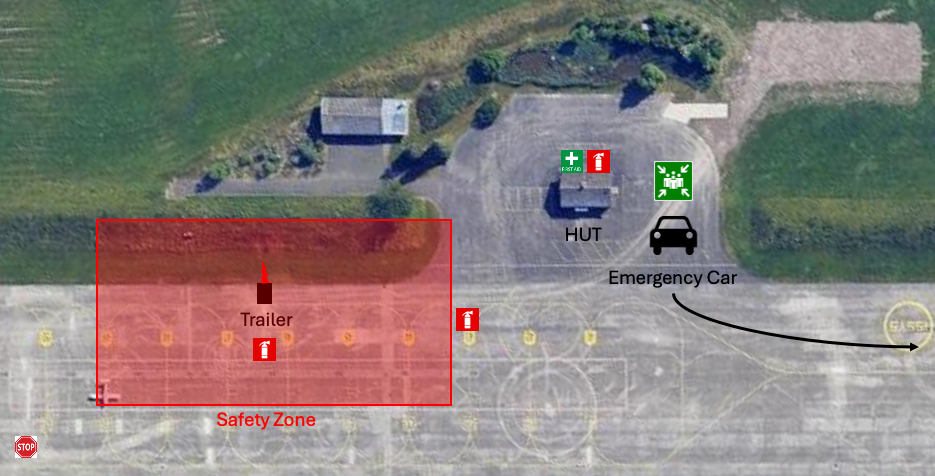
\includegraphics[width=\textwidth]{assets/location_map.png}
    \caption{Site map of the test location}
    \label{fig:location-plan}
\end{figure}

\newpage

\begin{figure}[h]
    \centering
    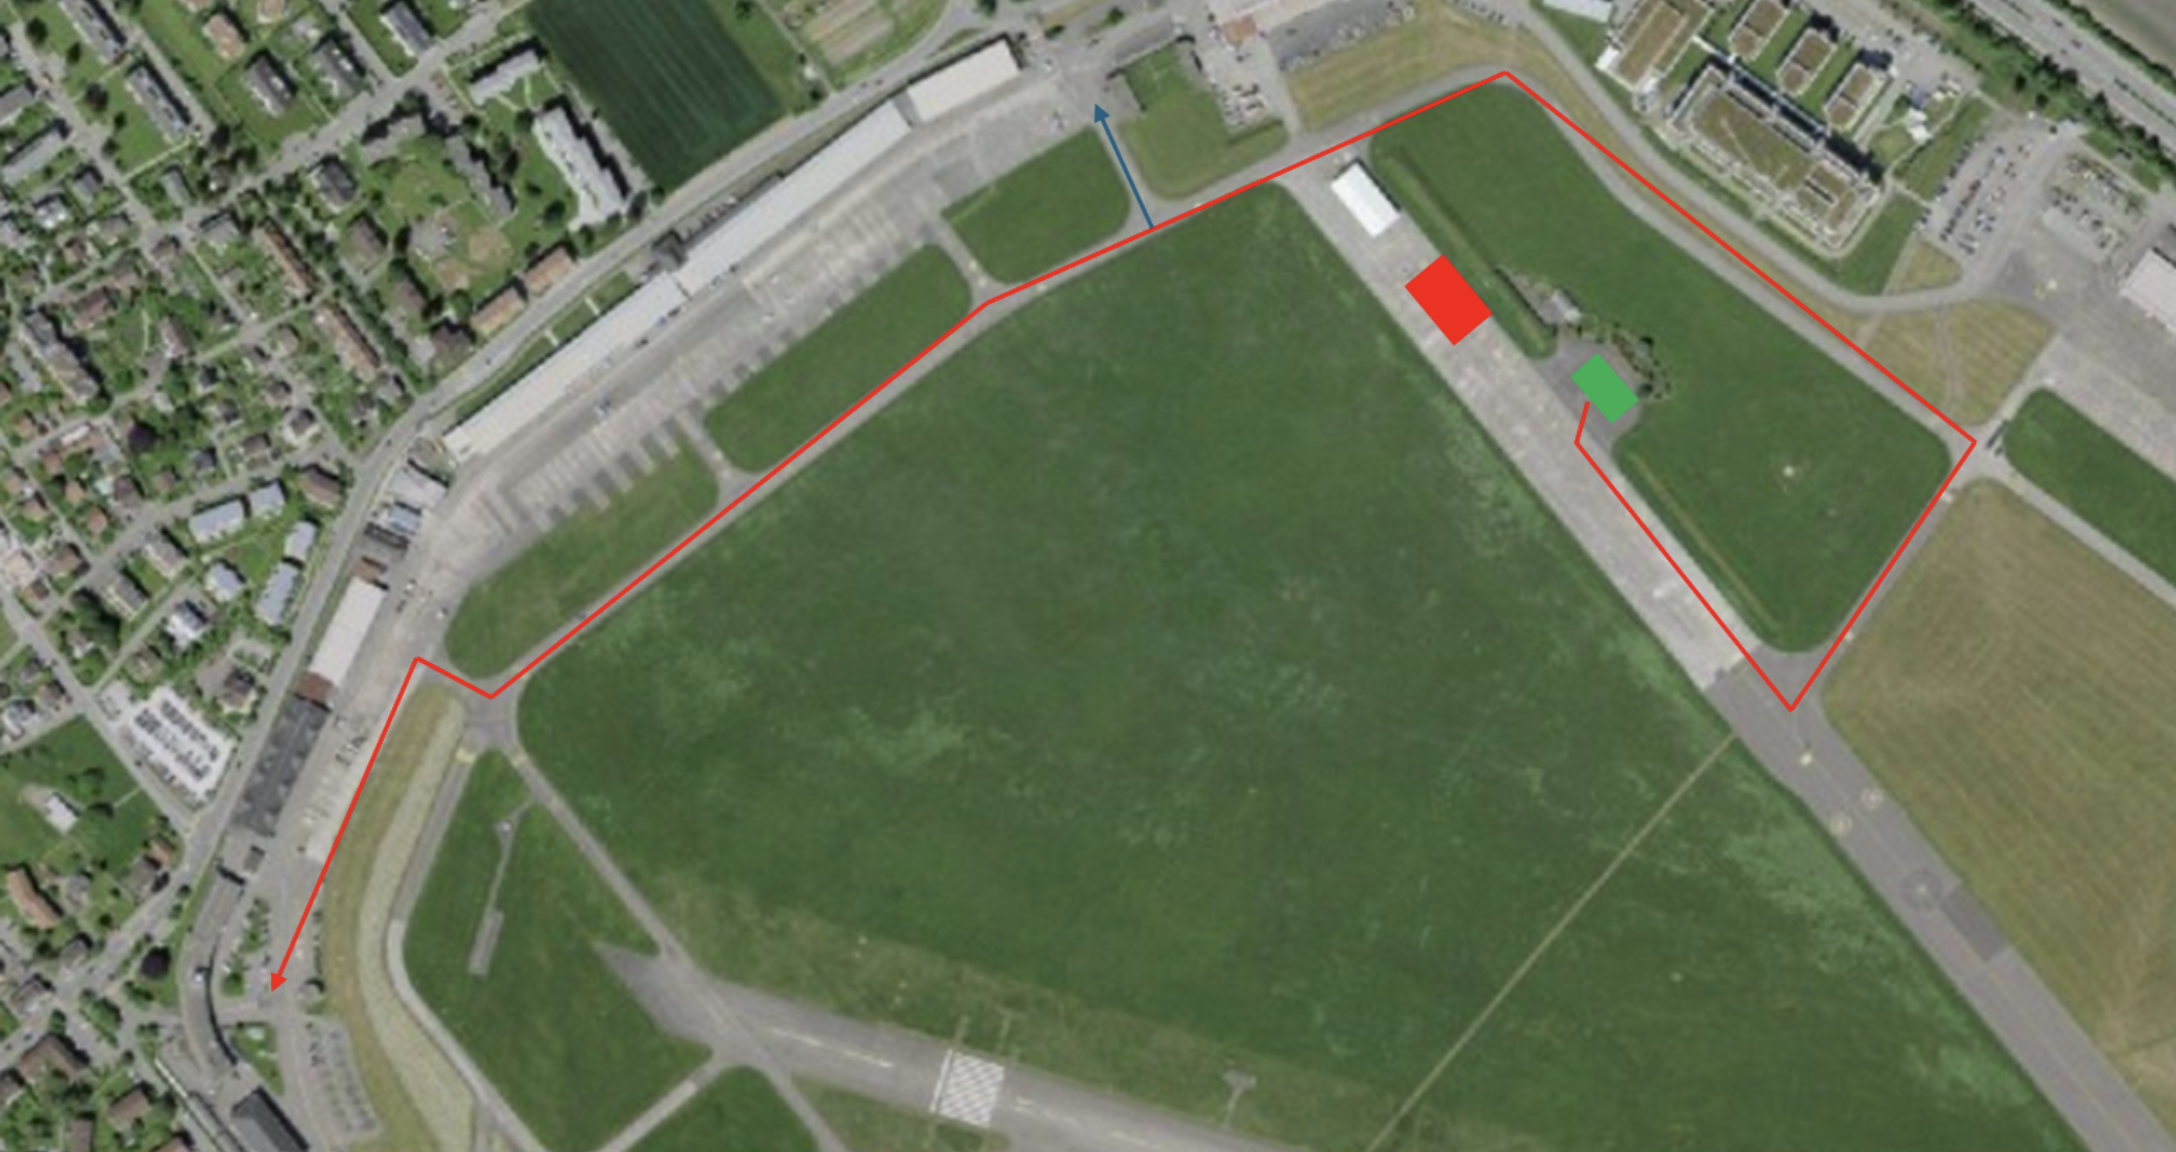
\includegraphics[width=\textwidth]{assets/emergency_route.png}
    \caption{Emergency route}
    \label{fig:emergency-route}
\end{figure}

\section{Equipment}
Every person has to wear a warning vest according to their role at all times during testing operations. The color code displayed in table \ref{tab:color-code} is used.
\begin{table}[h]
    \caption{Warning Vest Color Code}
    \label{tab:color-code}
    \begin{tabularx}{0.9\textwidth}{|X|X|X|X|}
        \hline
        \cellcolor{cyan} Test Conductor & \cellcolor{green} Safety Officer & \cellcolor{orange} Engineers in charge (determined in role assignment) & \cellcolor{yellow} Visitors, Remaining Engineers, Team Members \\ \hline
    \end{tabularx}
\end{table}
The safety equipment is stored in the entrance of the HUT. The wearing of provided safety equipmentas foreseen in the operating procedures is mandatory.
\begin{table}[h]
    \caption{Safety Equipment}
    \label{tab:safety-equipment}
    \begin{tabularx}{0.9\textwidth}{|c|X|X|}
        \hline
        \rowcolor{tableHeaderColor} \textbf{Amount} & \textbf{Equipment} & \textbf{Comment} \\ \hline
        2 & Fire extinguisher & ABC-Pulver (in HUT and behind wall see Figure \ref{fig:location-plan}) \\ \hline
        2 & Fire extinguisher & CO2 (class B next to trailer) \\ \hline
        1 & First aid kit & Located in the HUT \\ \hline
        1 & Emergency car & Parked on the west side of the HUT and open, car key and gate key on driver's seat \\ \hline
        2 & Blue warning vest & \\ \hline
        2 & Green warning vest & \\ \hline
        10 & Yellow warning vest & \\ \hline
        6 & Orange warning vest & \\ \hline
        8 & Safety goggles & \\ \hline
        4 & Face shield & \\ \hline
        6 & Pair of safety shoes & \\ \hline
        2 & Pair of cold-resistant gloves & For handling gas and LOX \\ \hline
        1 & Blast shield & \\ \hline
        10 & Ear protection & \\ \hline
        2 & Cold-resistant faceshield & \\ \hline
        8 & Work gloves & \\ \hline
        2 & Barrier tape & \\ \hline
    \end{tabularx}
\end{table}
\newpage
\section{Behaviour during test procedure}
The test conductor has the lead during the whole test operation and therefore gives the orders, which shall be obeyed. The safety officer supervises the actions of the test conductor and the team and makes sure that the tests are executed according to the procedures. The safety officer can stop the operations at any time he considers proceeding with the test as dangerous. \\
\noindent
If during the test procedure an anomaly occurs or if there is an insecurity, the test participants are requested to inform the test conductor and the safety officer immediately. \\
\noindent
The attendees are not allowed to take photos and record video material. A pre-determined photographer will take pictures and video footage. The publishing of this material via social media or other channels is strictly forbidden. All to be published material must be checked and approved by the Airfield Dübendorf on request of team HEPHAESTUS. \textbf{Please do not contact the Airfield on your own}. \\
\noindent
By signing the HEP\_GL\_SafetySignature you agree that during the tests pictures of you will be taken and used for internal purposes (photo gallery on website, flyer, Instagram, LinkedIn). If you do not agree, please contact the project manager or the safety officer during the briefing.

\section{Behaviour in case of an emergency} \label{emergency-behaviour}
In case of an emergency or an unexpected system state, the contingency procedures (shown in table \ref{tab:contingency-procedures}) must be followed. Participants will be informed about the location of the contingency procedures during the briefing and installation according to the Firing Conduction.
\begin{table}[h]
    \caption{Contingency Procedures}
    \label{tab:contingency-procedures}
    \begin{tabularx}{0.9\textwidth}{|X|}
        \cellcolor{blue} \textcolor{white}{General} \\ \hline
        HEP\_CP\_GEN\_Injury\_XX \\ \hline
        HEP\_CP\_GEN\_Fire\_XX \\ \hline
        HEP\_CP\_GEN\_Trespassing\_XX \\ \hline
        \cellcolor{orange} PSS \\ \hline
        HEP\_CP\_PSS\_Leakage\_XX \\ \hline
        HEP\_CP\_PSS\_Overpressure\_XX \\ \hline
        HEP\_CP\_PSS\_BottleValve-Anomaly\_XX \\ \hline
        HEP\_CP\_PSS\_NoisesHissing\_XX \\ \hline
        \cellcolor{yellow} DACS \\ \hline
        HEP\_CP\_DACS\_PowerLoss\_XX \\ \hline
        HEP\_CP\_DACS\_ConnectionLoss\_XX \\ \hline
        HEP\_CP\_DACS\_ValveAnomalies\_XX \\ \hline
    \end{tabularx}
\end{table}
All attendees are guided to stay calm and to avoid panicking. In such a situation, communication needs to be reduced to the minimum / essential only. The safety officer or his substitute leads through all emergency situations supported by the test conductor. The roles of emergency drivers and emergency assistants are assigned already in advance and are clearly stated in the operating procedures and will be communicated during the briefing. The replacement in the event of a role failure is defined in the respective operating procedure and also clearly announced during the briefing. \\
\noindent
In any situation, the hazards must be considered before providing assistance. Particularly, the HUT must not be left without prior consideration of the state of the system! \\
\noindent
As soon as the situation allows it, the safety officer will inform Roger Gisler (Airfield Dübendorf), Chloé Pilloud (ARIS). Contacting a technical expert (Bruno Berger) can also be helpful in situations where expert advice or a technical assessment is needed. 
\end{document}